\section{Vorbereitende Rechnungen}
\label{sec:vorbereitung}
%
Vorbereitend zur Durchführung des Versuches werden die zu untersuchenden Übergänge zunächst theoretisch untersucht. Dazu sind im Folgenden die Energiedifferenzen sowie die berechneten Lande-Faktoren aufgeführt.
%
\subsection{Die rote Linie der Cd-Lampe}
%
Die Übergänge der Elektronen, welche die rote Linie erzeugen sind jene von~$^{1}D_2$ nach~$^{1}P_1$. Die zu den beiden Zuständen gehörenden Quantenzahlen sind in Tabelle~\ref{tab:rot_cd} aufgeführt. Dort wird auch deutlich, dass es sich hierbei um den normalen Zeeman-Effekt handelt, da beide Zustände den Spin $0$ besitzen. Der Lande-Faktor ist hier für alle Zustände $g=1$. Mögliche Übergänge zwischen diesen beiden Niveaus sind in Abbildung~\ref{fig:therm_rot} dargestellt. Die aus Gleichung~\eqref{eq:dE_norm} bestimmten Energiedifferenzen der verschiedenen Übergänge sind in Tabelle \ref{tab:rot_cdE} aufgeführt.
%
\begin{figure}
    \centering
    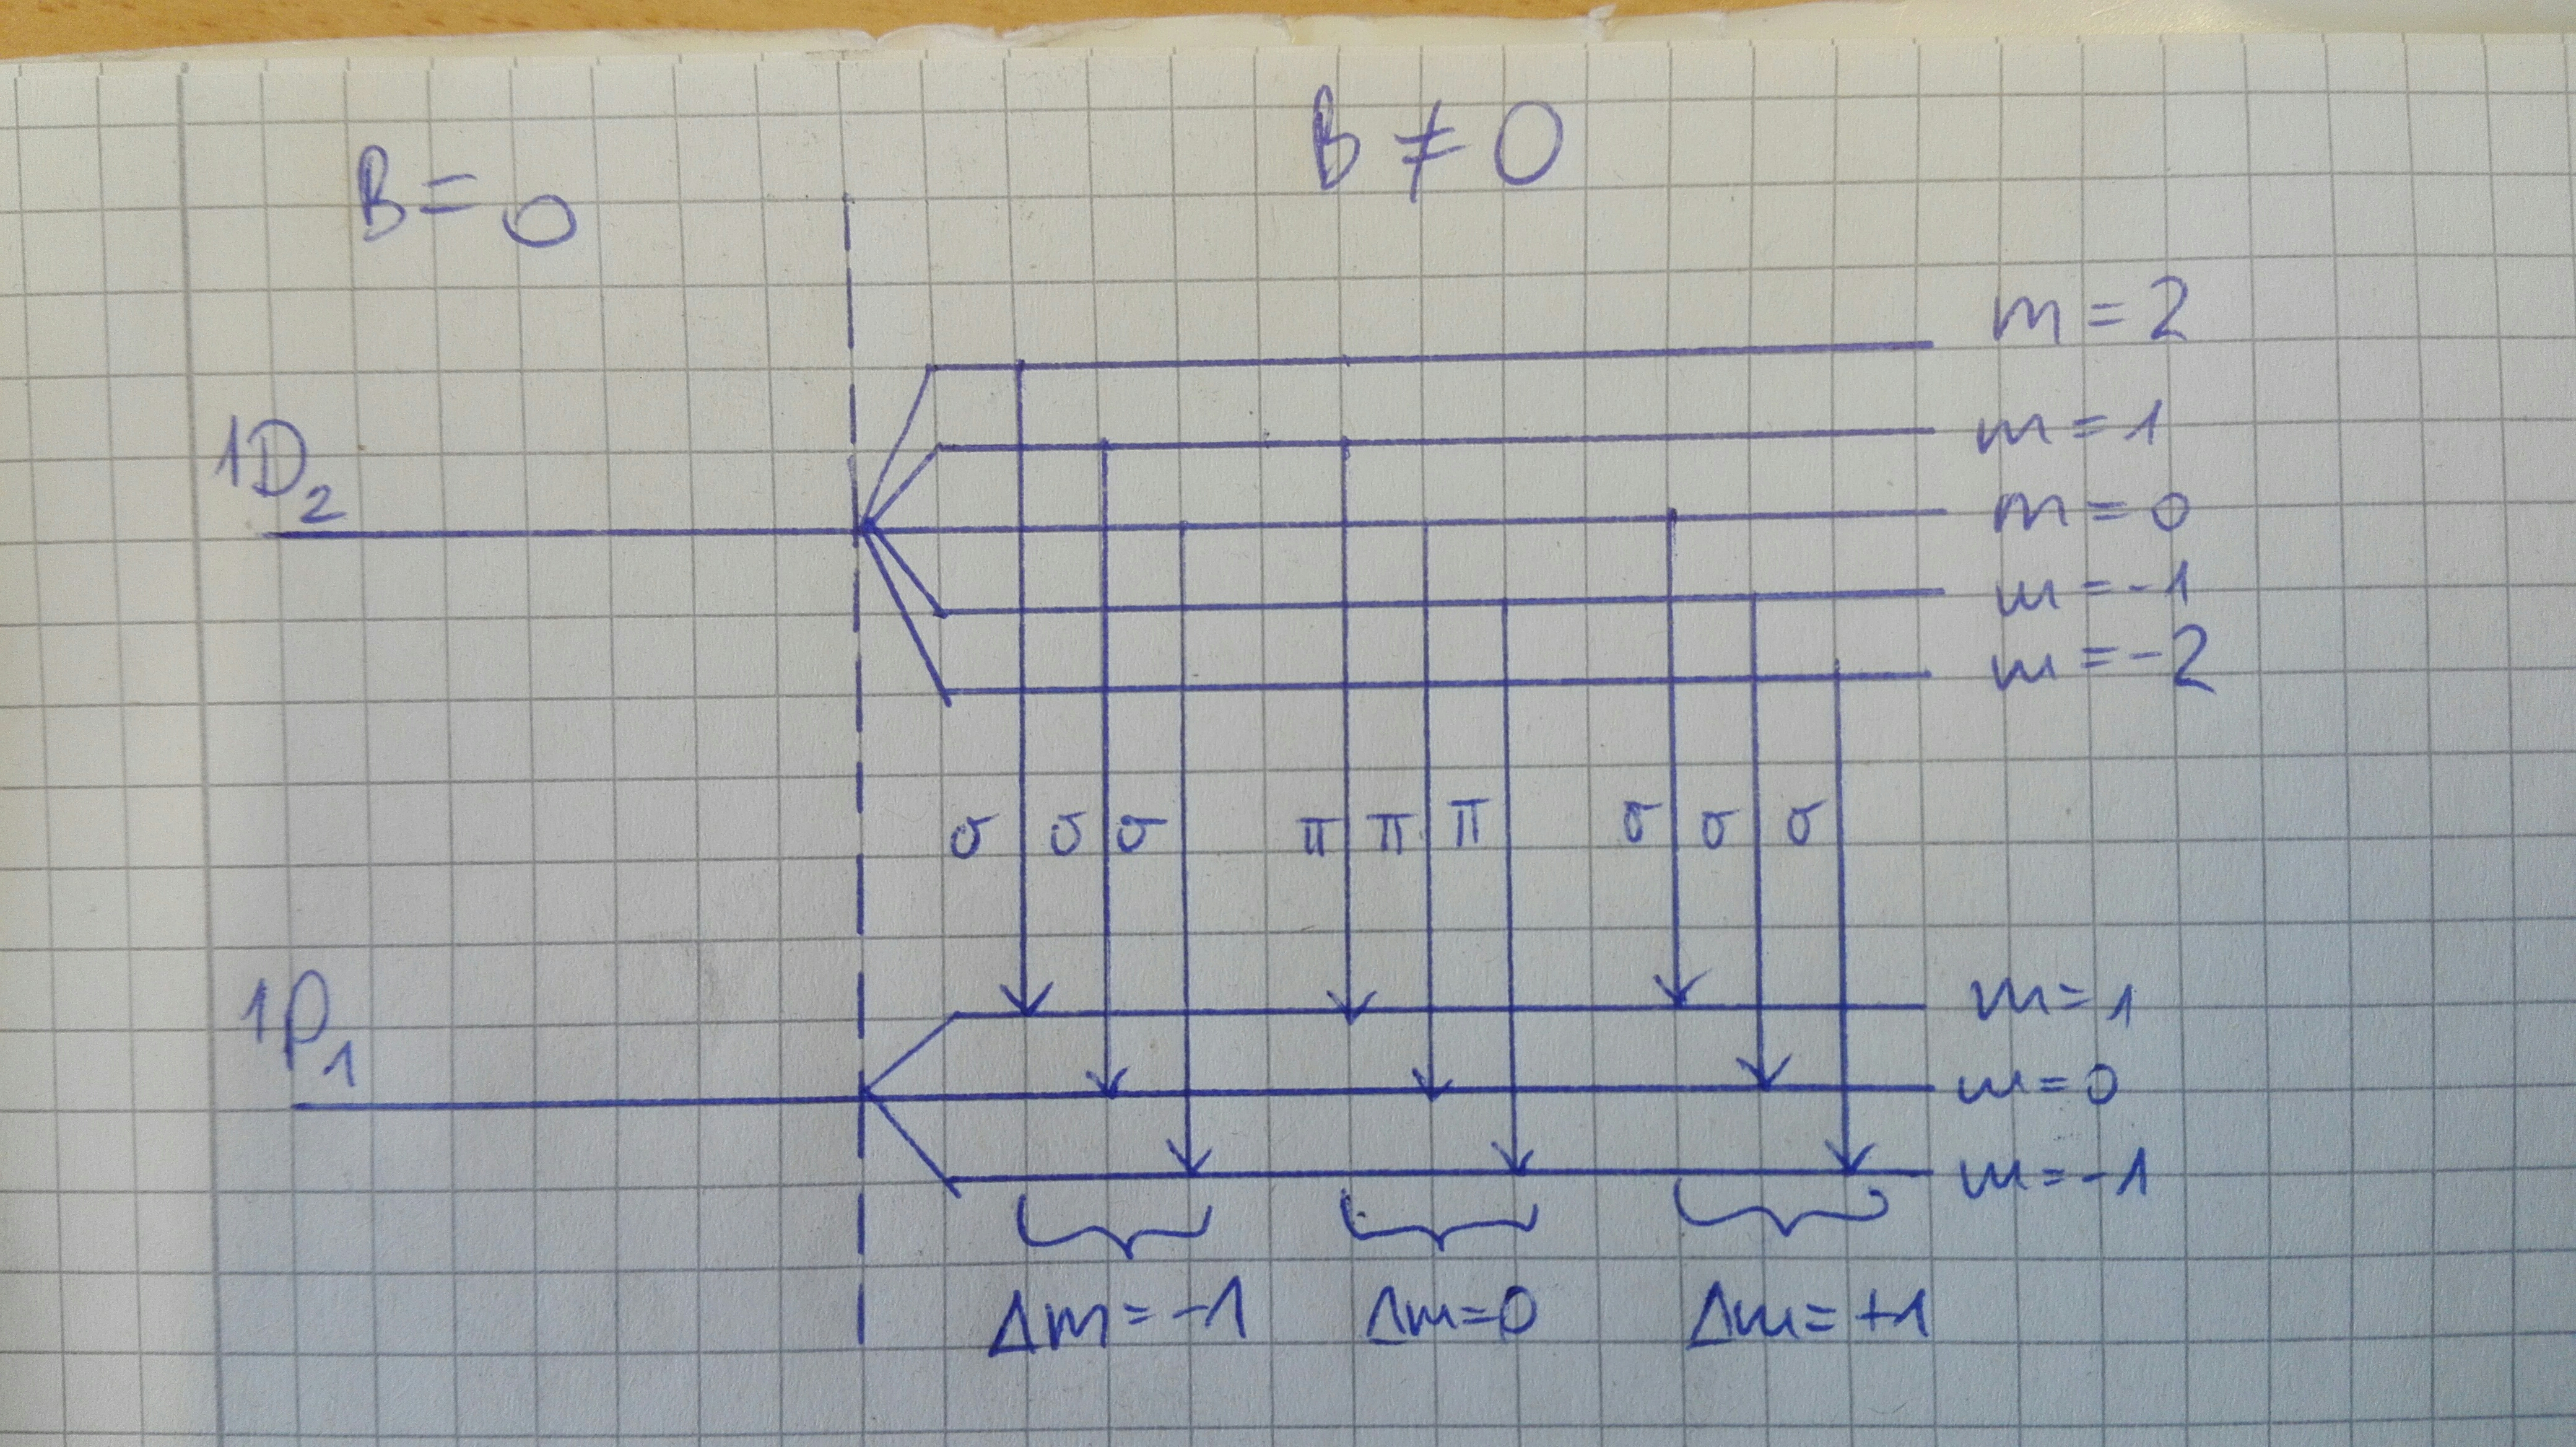
\includegraphics[width=0.8\textwidth]{figure/thermschema_rot.jpg}
    \caption{Termschema der roten Linie.}
    \label{fig:therm_rot}
\end{figure}
%
\begin{table}[H]
    \centering
    \caption{Quantenzahlen der Übergänge.}
    \begin{tabular}{cccccc}
        \toprule
    {} & {$L$}  & {$J$}  & {$S$} & {$m$} & {$g$} \\
		\midrule
	  $^{1}D_2$ & 2 & 2 & 0 & $-2,-1,0,1,2$ & 1 \\
    $^{1}P_1$ & 1 & 1 & 0 & $-1,0,1$ & 1 \\
    \bottomrule
	\end{tabular}
    \label{tab:rot_cd}
\end{table}
%
\begin{table}[H]
    \centering
    \caption{Energieaufspaltung der Zeeman-Linien.}
    \begin{tabular}{cc}
        \toprule
    {Übergang} & {$\mathup{\Delta}E$} \\
		\midrule
	  $\mathup{\Delta}m=-1$ & $-\mu_\mathup{B}B$ \\
    $\mathup{\Delta}m=0$ & 0 \\
    $\mathup{\Delta}m=1$ & $\mu_\mathup{B}B$ \\
    \bottomrule
	\end{tabular}
    \label{tab:rot_cdE}
\end{table}
%
\subsection{Die blaue Linie der Cd-Lampe}
%
Die Übergänge der Elektronen, welche die blaue Linie erzeugen sind jene von~$^{3}P_1$ nach~$^{3}S_1$. Die zu den beiden Zuständen gehörenden Quantenzahlen sind in Tabelle~\ref{tab:blau_cd} aufgeführt. Die Zustände werden durch ein anliegendes Magnetfeld aufgespalten. Durch die beiden gleich von Null verschiedenen Spins wird auch deutlich, dass es sich hierbei um den anomalen Zeeman-Effekt handelt. Der Lande-Faktor ist hier für alle Zustände $g\neq1$. Mögliche Übergänge zwischen diesen beiden Niveaus sind in Abbildung~\ref{fig:therm_blau} dargestellt. Die aus Gleichung~\eqref{eq:dE_ano} bestimmten Energiedifferenzen der verschiedenen Übergänge sind in Tabelle \ref{tab:blau_cdE} aufgeführt.
%
\begin{figure}
    \centering
    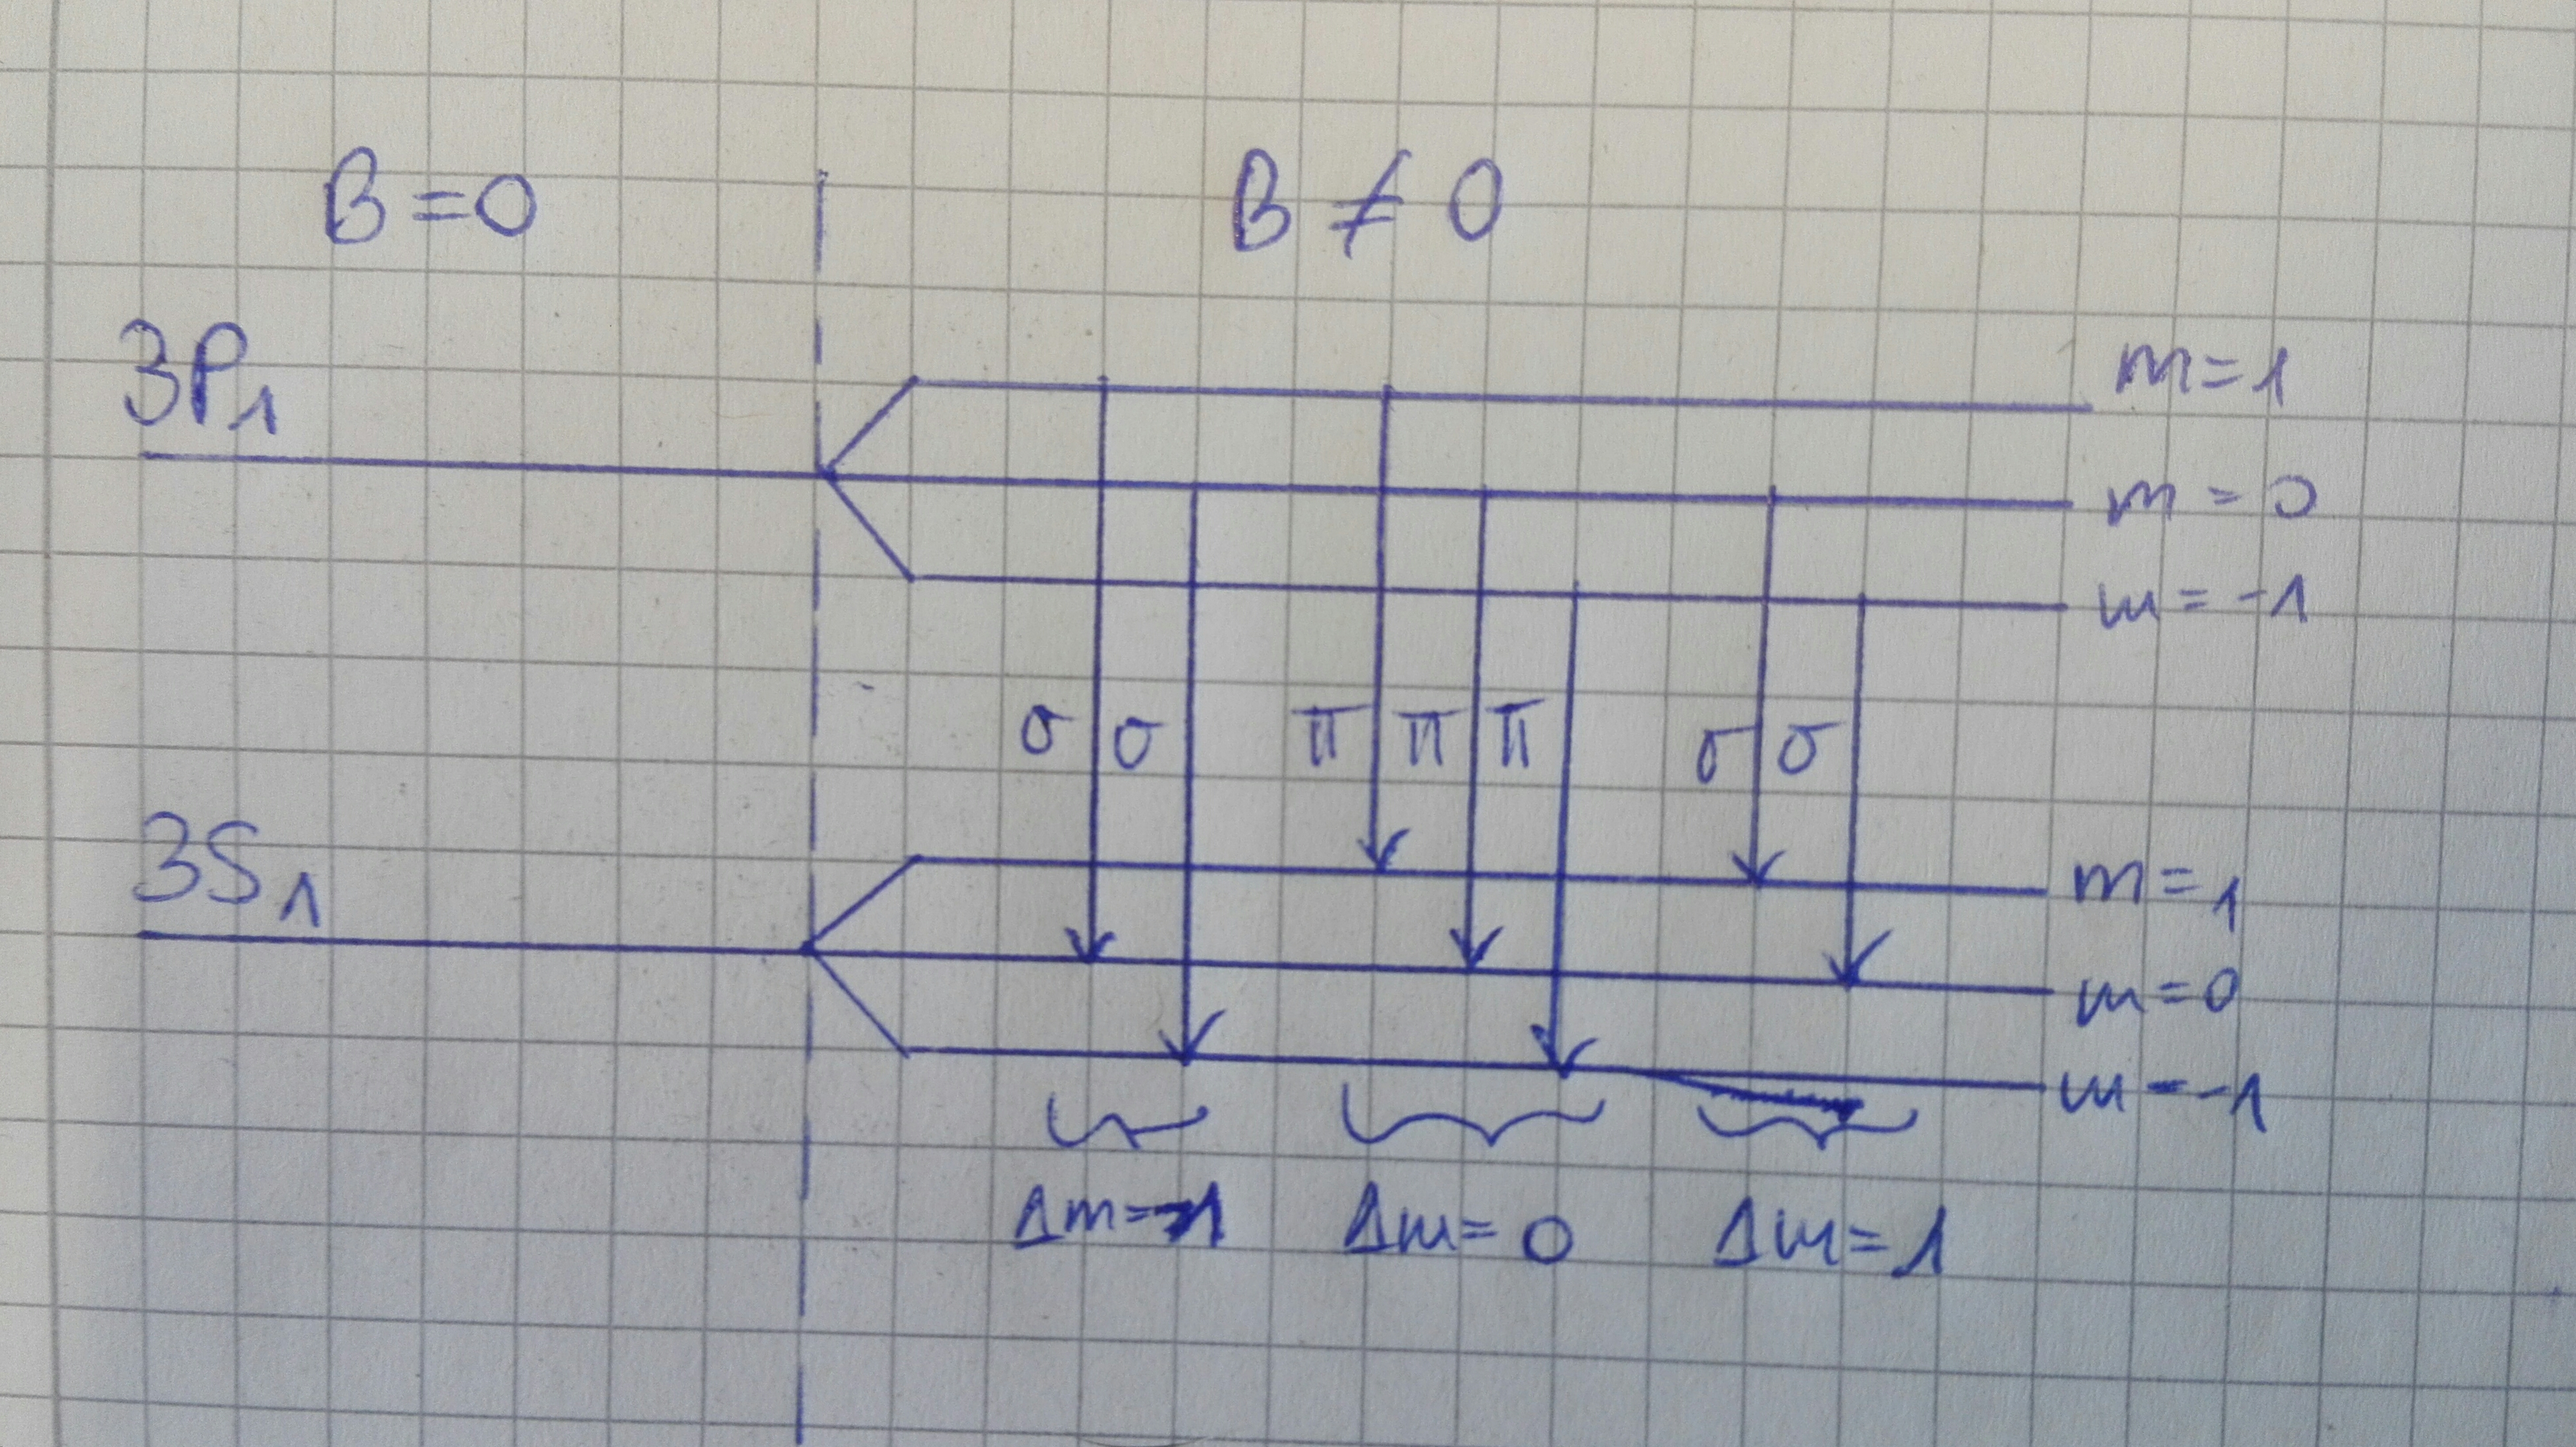
\includegraphics[width=0.8\textwidth]{figure/thermschema_blau.jpg}
    \caption{Termschema der blauen Linie.}
    \label{fig:therm_blau}
\end{figure}
%
\begin{table}[H]
    \centering
    \caption{Quantenzahlen der Übergänge.}
    \begin{tabular}{cccccc}
        \toprule
    {} & {$L$}  & {$J$}  & {$S$} & {$m$} & {$g$} \\
		\midrule
	  $^{3}P_1$ & 1 & 1 & 1 & $-1,0,1$ & 1,5 \\
    $^{3}S_1$ & 0 & 1 & 1 & $-1,0,1$ & 2 \\
    \bottomrule
	\end{tabular}
    \label{tab:blau_cd}
\end{table}
%
\begin{table}[H]
    \centering
    \caption{Energieaufspaltung der Zeeman-Linien.}
    \begin{tabular}{ccc}
        \toprule
    {Übergang} & {$m_1\rightarrow m_2$}  & {$\mathup{\Delta}E$} \\
		\midrule
    \multirow{2}{*}{$\mathup{\Delta}m=-1$}& 1\rightarrow 0 & $1,5\mu_\mathup{B}B$  \\
	   & 0\rightarrow -1  & $2\mu_\mathup{B}B$ \\ \hline
    \multirow{3}{*}{$\mathup{\Delta}m=0$}& 1\rightarrow 1 & $-0,5\mu_\mathup{B}B$  \\
 	   & 0\rightarrow 0  & $0$ \\
     & -1\rightarrow-1 & $0,5\mu_\mathup{B}B$ \\ \hline
    \multirow{2}{*}{$\mathup{\Delta}m=+1$}& 0\rightarrow 1 & $-2\mu_\mathup{B}B$  \\
 	   & -1\rightarrow 0  & $-1,5\mu_\mathup{B}B$ \\
    \bottomrule
	\end{tabular}
    \label{tab:blau_cdE}
\end{table}
%
\subsection{Zusammenfassung der Ergebnisse}
%
Zusammenfassend ergeben sich für die Übergänge der verschiedenen Linien die in Tabelle~\ref{tab:lande} aufgeführten Ergebnisse für die Lande-Faktoren $|g|$. Diese sollen im Versuch experimentell validiert werden.
%
\begin{table}[H]
    \centering
    \caption{Theoretische Vorhersage für $|g|$.}
    \begin{tabular}{ccc}
    \toprule
    {Linie} & {rot}  & {blau} \\
		\midrule
    $\sigma$ & 1 & 1,75  \\
	  $\pi$ & 0 & 0.5 \\
    \bottomrule
	\end{tabular}
    \label{tab:lande}
\end{table}
